% This is samplepaper.tex, a sample chapter demonstrating the
% LLNCS macro package for Springer Computer Science proceedings;
% Version 2.20 of 2017/10/04
%
\documentclass[a4paper]{llncs}
%
\usepackage{amsmath,amssymb}
\usepackage{graphicx}
% Used for displaying a sample figure. If possible, figure files should
% be included in EPS format.
%
% If you use the hyperref package, please uncomment the following line
% to display URLs in blue roman font according to Springer's eBook style:
% \renewcommand\UrlFont{\color{blue}\rmfamily}
\usepackage[english]{babel}
\usepackage[autostyle]{csquotes}
\usepackage[sorting=ynt,sortcites=true,backend=bibtex8,doi=false,maxnames=4,isbn=false,firstinits=true]{biblatex}
\addbibresource{reference}

\usepackage{hyperref}
\hypersetup
{
  bookmarks       = true,
  unicode         = true,
  pdftitle        = "Type Flattening Obfuscation",
  pdfauthor       = "Ta Thanh Dinh", %auteur du document
%   pdfsubject      = "A Conceptual Approach for Message Format Extraction",
  pdftoolbar      = true, %barre d'outils non visible
  pdfmenubar      = true, %barre de menu visible
  pdfhighlight    = /O, %effet d'un clic sur un lien hypertexte
  colorlinks      = true, %couleurs sur les liens hypertextes
%   pdfpagemode = None, %aucun mode de page
%   pdfpagelayout = SinglePage, %ouverture en simple page
  pdffitwindow    = true, %pages ouvertes entierement dans toute la fenetre
  linkcolor       = red, %couleur des liens hypertextes internes
  citecolor       = green, %couleur des liens pour les citations
  urlcolor        = cyan, %couleur des liens pour les url
%   pagebackref=true
%   bookmarksdepth  = 3
}

\usepackage{listings}
\lstset{basicstyle=\small\ttfamily,showspaces=false,frame=tb}
\lstloadlanguages{C,C++,[x86masm]Assembler}

% \usepackage{cleveref}
% \usepackage{adjustbox}
\usepackage[strict]{changepage}

\begin{document}
%
\title{Type Flattening Obfuscation}
%
%\titlerunning{Abbreviated paper title}
% If the paper title is too long for the running head, you can set
% an abbreviated paper title here
%
\author{Ta Thanh Dinh}
%
\authorrunning{Ta Thanh Dinh}
% First names are abbreviated in the running head.
% If there are more than two authors, 'et al.' is used.
%
\institute{
	\email{tathanhdinh@gmail.com}}
%
\maketitle              % typeset the header of the contribution
%
\begin{abstract}
	Beside data and control flow, high-level types are also important in program analysis,
	indeed type recovery is an essential step in binary code decompilation.
	For the purpose of anti-decompilation, the paper presents a novel obfuscation
	technique which makes types become harder to be reconstructed.

	% High-level type reconstruction is an important step in machine code decompilation.
	% Researchers show possibilities of mapping untyped machine-dependent
	% primitives into types of a C-like type system.


	% We show that the techniques used for type reconstruction can be bypassed,
	% and we claim that the bypass is always possible given \emph{semantics gap} between
	% type systems of high-level and machine language.
	% \keywords{First keyword  \and Second keyword \and Another keyword.}
\end{abstract}
%
%
%
\section{Introduction}
An important step in binary code \emph{decompilation}~\cite{cifuentes_reverse_1994} is to
detect high-level objects (e.g. functions, variables) from low-level machine dependent
objects~\cite{balakrishnan_divine_2007} (e.g. registers, raw memory accesses, machine
instructions) before annotate them with types of the "assumed" original language.
In a statically typed language like C, the compiler does not preserve the high-level
type information in the generated machine code,
% Because most of information about high-level types is lost in compilation,
% the machine code
then the \emph{type recovery} (or type reconstruction) from machine code requires
special techniques, a survey up until 2015 can be referenced in~\cite{caballero_type_2016}.

In the opposite direction, binary code \emph{obfuscation} is to make the decompilation (or in
general code analysis) harder. Since the data and control flow are principal elements for the
program analysis, current obfuscation methods~\cite{collberg_surreptitious_2009} focus mostly
on them. But to the best of our knowledge, there is still no explicit effort in obfuscating
high-level types. There would be several reasons for this lack of effort.

\emph{First}, type obfuscation is unsurprisingly a side effect of data or control flow obfuscation.
Indeed, type reconstruction algorithms need both data and control flow to build type constraints,
if any of them is hidden
then the algorithms cannot work correctly. Or if the function boundary is not found
(because of anti-disassembing tricks, for example), then high-level objects cannot be recognized.
\emph{Second}, high-level types seem too coarse to be worthy
of being protected, in many cases just knowing certain values of the input which make the program
exploitable is enough. But knowledge about types expands attack surfaces because more analysis
can be proceeded, beside decompilation see the survey~\cite{caballero_type_2016} for a
more complete list.
% We exploit the \emph{semantics gap}


\section{Type flattening compiler}
We present \emph{uCc}, an open source C compiler that explicitly obfuscates high-level types, \emph{uCc}'s
objective is to make reconstructing C types from machine codes harder.
The compiler is implemented in Rust, the source code and a brief user guide are given at (cite); different
from other code obfuscation implementations, \emph{uCc} uses cranelift~\cite{noauthor_cranelift_nodate} as
backend.

Our effort is to attack the core of type reconstruction algorithms,
these are the data flow used to build type constraints, and the \emph{semantic gap} between types in the high-level language and their
representations in the low-level machine code.
Beside custom tricks which would be fully presented in another paper, \emph{uCc} uses extensively
obfuscation transformations based on Mixed Boolean Arithmetic expressions~\cite{eyrolles_obfuscation_2017,zhou_information_2007}.
To make some code diversity, the compiler is \emph{probabilistic}: given a source
code, \emph{uCc} generates each time a different (but computationally equivalent) output machine code.

We test outputs of \emph{uCc} against some decompilers (the test suite is available at
the repository). Table~\ref{description} describes briefly
tested functions and their types in source codes, table~\ref{flattening} shows results of using
$4$ decompilers to decompile binaries generated by \emph{uCc}.
No one between tested decompilers can recognize the precise signature of tested functions.
Basically, any argument is assigned by either \texttt{int64} or \texttt{uint64},
the highest types in the \emph{conversion rank} of integer types, we call this effect \emph{type flattening}.

We may note that if the tested functions are
compiled by, \emph{clang} for example, then their signatures can be recognized precisely
by the decompilers. Last but not least, \emph{uCc} makes no effort in making disassembling or function
boundary detection hard. Indeed, functions in tested binaries are perfectly detectable,
disassemblable and decompilable.

\begin{table}
	\begin{center}
		\caption{Functions and original types}\label{description}
		\begin{tabular}{|l|l|}
			\hline
			Description & Function type \\
			\hline
			identity & \texttt{int id(int)} \\
			\hline
			division & \texttt{int div(short, char)} \\
			\hline
			modular & \texttt{char mod(short, char)} \\
			\hline
			increase $p \leftarrow p + 1$ then dereference & \texttt{int inc\_deref(int *p)} \\
			\hline
			strlen  & \texttt{int slen(char* s)} \\
			\hline
			sdbm hash & \texttt{int sdbm(char *s)} \\
			\hline
			djb2 hash & \texttt{int djb2(char *s)} \\
			\hline
			sum of array $a$ & \texttt{long sum(short *a, int n)} \\
			\hline
			$n$-th fibonaci number (recursive impl.) & \texttt{int fibo(int n)} \\
			\hline
			num. of steps until $n \rightsquigarrow 1$ (Collatz's conj.)  & \texttt{int collatz(int n)} \\
			\hline
		\end{tabular}
	\end{center}
\end{table}

\begin{table}
	\begin{adjustwidth}{-6.21in}{-5.95in}
		\begin{center}
			% \centering
			\caption{Type flattening effect}\label{flattening}
			% \begin{adjustbox}{max width=1.5\textwidth}
			\begin{tabular}{|l|l|l|l|l|}
				\hline
				Original type & Hex-Rays & JEB & Ghidra & Snowman \\
				\hline
				\texttt{int id(int)} & \texttt{int64 id(int64)} & \texttt{ulong id(ulong)} &
				\texttt{ulong id(void)} & \texttt{int64 id(int64)} \\
				\hline
				\texttt{short div(short, char)} & \texttt{int64 div(uint64, uint64)} & \texttt{div\_t div(int, int)} &
				\texttt{div\_t div(int, int)} & \texttt{int64\_t div(int64, int64)} \\
				\hline
				\texttt{char mod(short, char)} & \texttt{int64 mod(int64, int64)} & \texttt{ulong mod(ulong, ulong)} &
				\texttt{ulong mod(void)} & \texttt{int64 mod(int64, int64)} \\
				\hline
				\texttt{int inc\_deref(int*)} & \texttt{int64 inc\_deref(int64)} & \texttt{ulong inc\_deref(ulong)} &
				\texttt{ulong inc\_deref(undefined8)} & \texttt{int64 inc\_deref(uint64)} \\
				\hline
				\texttt{int slen(char*)} & \texttt{int64 slen(int64)} & \texttt{ulong slen(ulong)} &
				\texttt{ulong slen(undefined8)} & \texttt{int64 slen(uint64)} \\
				\hline
				\texttt{int sdbm(char*)} & \texttt{int64 sdbm(uint64)} & \texttt{ulong sdbm(ulong)} &
				\texttt{ulong sdbm(undefined8)} & \texttt{int64 sdbm(uint64)} \\
				\hline
				\texttt{int djb2(char*)} & \texttt{int64 djb2(uint64)} & \texttt{ulong djb2(ulong)} &
				\texttt{ulong djb2(undefined8)} & \texttt{int64 djb2(uint64)} \\
				\hline
				\texttt{long sum(short*, int)} & \texttt{int64 sum(int64, uint64)} &
				\texttt{ulong sum(ulong, ulong)} & \texttt{undefined8 sum(undefined8)} & \texttt{int64 sum(uint64, int64)} \\
				\hline
				\texttt{int fibo(int)} & \texttt{int64 fibo(uint64)} & \texttt{ulong fibo(ulong)} &
				\texttt{ulong fibo(undefined8)} & \texttt{int64 fibo(int64)} \\
				\hline
				\texttt{int collatz(int)} & \texttt{int64 collatz(int64)} & \texttt{ulong collatz(ulong)} &
				\texttt{ulong collatz(undefined8)} & \texttt{int64 collatz(int64)} \\
				\hline
			\end{tabular}
		\end{center}
	\end{adjustwidth}
\end{table}

% \begin{table}
% \caption{Table captions should be placed above the
% tables.}\label{tab1}
% \begin{tabular}{|l|l|l|}
% \hline
% Heading level &  Example & Font size and style\\
% \hline
% Title (centered) &  {\Large\bfseries Lecture Notes} & 14 point, bold\\
% 1st-level heading &  {\large\bfseries 1 Introduction} & 12 point, bold\\
% 2nd-level heading & {\bfseries 2.1 Printing Area} & 10 point, bold\\
% 3rd-level heading & {\bfseries Run-in Heading in Bold.} Text follows & 10 point, bold\\
% 4th-level heading & {\itshape Lowest Level Heading.} Text follows & 10 point, italic\\
% \hline
% \end{tabular}
% \end{table}

% \section{Introduction}
% Binary code type recovery is to restore high-level type information of variables,
% functions from machine codes. It is useful for reverse code engineering (e.g.
% decompilation) or static binary rewriting/instrumentation, just to name a few.
% Type recovery is available in several binary analysis
% tools~\cite{noauthor_hex-rays_nodate, noauthor_jeb_nodate, noauthor_ghidra_nodate}
% as a result of machine code decompilation. Academic research includes the classic
% paper of Mycroft~\cite{mycroft_type-based_1999} which is probably the first work
% on the domain, though earlier ideas~\cite{shivers_data-flow_1990} have been used
% to recover types of programs in Scheme - a dynamically typed language.
% Lee et al.~\cite{lee_tie_2011} extend Mycroft's work by introducing a form of
% subtyping based on C's integer conversion rank, but lack of recursive type.
% Polymorphic Type Inference for Machine Code.
% Caballero and Lin give a survey~\cite{caballero_type_2016} for research up until 2015.
% Recent directions are using machine learning~\cite{maier_typeminer_2019} or statistical
% language model~\cite{katz_estimating_2016}, which are out of scope of the paper.
% All approaches tend to output a C-like type system.

% Basically, the binary code type recovery starts by detecting high-level objects from
% machine-dependent primitives: local variables are stored in function stack frame,
% parameters are passed from registers, see~\cite{balakrishnan_wysinwyx_2007} for related techniques.
% Type constraints are generated gradually through the \emph{low-level use} of objects.
% The system of constraints is solved then, each object is assigned a certain
% (polymorphic) type.

% This bird view may give off an impression that the
% binary code type reconstruction is a well established research domain, incorrect results
% are because of foreign reasons: incorrect binary code disassembling,
% high-level variable detection, etc. But we claim that there are probably intrinsic problems.

% \emph{First}, there is a common agreement that type information is removed through
% compilation~\cite{lee_tie_2011,caballero_type_2016,lin_automatic_2010},
% but there is no explicit explication of why and how some type information is not needed,
% so removed, in machine codes. The result of reconstructing \emph{the most precise yet conservative}
% type~\cite{lee_tie_2011}, which may suggest the well-known
% \emph{principal types}~\cite{damas_principal_1982,hindley_principal_1969},
% is sound in a limited context only. Actually not all type
% information can be restored.

% \emph{Second}, though some techniques of data structure reverse
% engineering~\cite{caballero_type_2016, caballero_polyglot_2007} can be reused for
% type recovery, types do not always attach with storage specific primitives (for example
% \texttt{int} is some \texttt{32-bit} signed integer stored in a register or stack).
% The storage-based point of view is almost correct in low-level languages like C, it
% does not reveal the nature of types. In other languages, types can be
% zero-sized~\cite{noauthor_phantom_nodate}, another examples are
% \emph{regions}~\cite{grossman_region-based_2002} or \emph{units-of-measure}~\cite{kennedy_types_2010}
% which leave no storage imprint.

% \emph{Third}, current research uses some variants of
% \emph{Algorithm W}~\cite{milner_theory_1978,cardelli_basic_1987} to resolve type
% constraints in a C-like language. But the polymorphism in C is rather
% \emph{ad-hoc}~\cite{strachey_fundamental_2000}: some functions are
% trivially typed in C by casting, but not typeable in Hindley-Milner type system. This
% problem is remarked already in~\cite{mycroft_type-based_1999}, but unfortunately omitted in
% later extension~\cite{lee_tie_2011}. In real world, it is not rare to see type inconsistency in decompilation results
% of security tools.

% % used originally to
% % type check/inference for programs of Hindley-Milner's type system (abbr. HM).
% % While the supposed target is a C-like type system, some authors claim to replicate
% % the result of \emph{principal types}~\cite{damas_principal_1982,hindley_principal_1969}
% % by recovering \emph{the most precise yet conservative} type~\cite{lee_tie_2011}.
% % Such a result is sound in a limited context only, C's type system is not HM: there
% % are functions that are trivially typed in C by casting, but not typeable in HM's.
% % Actually, it is not rare to observe type inconsistency in decompilation results
% % of security tools.

% \paragraph{Contribution}
% We first discuss the type information loss in compilation and some cases
% where assigning a high-level \emph{type} for a low-level primitive
% is not possible. Though this part is not novel, we bring it to the context
% of binary code analysis to show limits of type reconstruction. Next, we present
% a proof-of-concept C compiler which tries to hide types from reconstruction techniques described
% in current researches.

% \section{Type information loss}
% Informally speaking, a type system is some set of constraints and rules to infer constraints
% on a program. The type system decides which are allowed or forbidden on the semantics of the language,
% for example adding two pointers is not allowed in C because this operation is semantically nonsense.
% Type helps avoid bugs as summarized in Milner's famous
% slogan~\textquote{well-type program cannot go wrong}~\cite{milner_theory_1978}.

% In statically typed languages, the compiler checks the type constraints then generates
% machine codes (we consider here only languages which generates machine codes), but then
% most of constraints are lost because they are not needed for running
% the program. There are at least two sources of
% information loss: \emph{type erasure} and \emph{data indistinguishability},
% happening at different phases of compilation.

% \subsection{Type erasure}
% \emph{Type erasure} means the "intensional" type of an object is hidden/inaccessible or
% completely removed in some context. It appears under several concepts: subtype substitution,
% generic specialization (or monomorphization), or boxing, just name a few. In some cases,
% e.g. subtype substitution, the (sub)type of the wrapped object does not completely removed,
% it is just not accessible in contexts where only behaviors of the super type are allowed.
% Such a case will not be discussed in the paper since we look at the low-level machine code.

% Once the program is type checked,
% % the type information is normally not needed for evaluation (i.e. running program),
% the compiler will select a consistent machine-dependent
% representation for each high-level type, this representation may only have little
% relation with the original type but it does not violate the fact that the program
% is checked, then safe.

% \begin{example}\label{exa:typed_enum}
% 	\texttt{C++}'s typed enum.

% 	\begin{lstlisting}[frame=lines, language={C++}]
% enum E { one = 1, two };
% void foo(enum E e) {
%   switch (e) {
%   case E::one:
%   case E::two:
%     printf("ok\n");
%     break;

%   default: assert(false);
%   }
% }

% enum E bar() {...return some enum E }

% int main() {
%   enum E e = bar(); foo(e);
%   return 0:
% }
% \end{lstlisting}

% 	The program is safe when type-checked: \texttt{assert(0)} will
% 	never be reached when the program runs. In machine code, we may observe that
% 	\texttt{foo} is a function accepting a \texttt{32-bit} signed integer, i.e. information about
% 	\texttt{enum E} type is erased. However there is no need to add runtime
% 	checking for the case where \texttt{foo} is passed an argument of value not in \texttt{enum E}
% 	(e.g. \texttt{3}), this case is eliminated by the compiler's type checker.
% \end{example}

% \subsection{Data indistinguishability}
% When generating binary code for a specific hardware/operating system, the compiler will
% use a consistent representation for low-level primitives (e.g. registers used in
% function parameters or return value, alignment for fields of aggregate types), so that
% the output binary can be used by other programs on the same system. It it possible that
% two types are distinguished at high-level but they have the same data representation
% at low-level.

% \begin{example}\label{exa:register_struct}
% 	Small struct passing.

% 	\begin{lstlisting}[frame=lines, language={C}]
% struct S { int a; int b; };
% int foo(struct S s) {
%   return s.a + s.b;
% }

% int bar(long long l) {
%   return (int)l + (int)(l >> 32);
% }
% \end{lstlisting}

% 	Under System V AMD64 ABI~\cite{lu_system_nodate}, the aggregate type \texttt{S}
% 	has class \texttt{INTEGER}: the argument \texttt{s} is passed just in register \texttt{rdi}.
% 	At the ABI level, \texttt{foo} and \texttt{bar} is interchangeable, but they are not at
% 	the type level.
% \end{example}

% \subsection{Untypeable}

% There is no type casting in Hindley-Milner's type system (abbr. HM), so when using a variant of
% \emph{Algorithm-W}~\cite{milner_theory_1978} for binary code type inference, the output (as a
% C program without type casting) may not exist: there are programs which are
% trivially typed in C, but not in HM.

% \begin{example}\label{exa:untypeable}
% 	Untypeable function.
% 	\begin{lstlisting}[frame=topline, language={C}]
% int foo(int i, int *f) {
%   return ((int (*)(int (*)(int, int*), int))f)(foo, i);
% }
% \end{lstlisting}
% 	Disassembled code:
% 	\begin{lstlisting}[frame=bottomline, language={[x86masm]Assembler}]
% 0x0     55                               push rbp
% 0x1     48 89 e5                         mov rbp, rsp
% 0x4     48 83 ec 10                      sub rsp, 0x10
% 0x8     89 7d fc                         mov [rbp-0x4], edi
% 0xb     48 89 75 f0                      mov [rbp-0x10], rsi
% 0xf     48 8b 45 f0                      mov rax, [rbp-0x10]
% 0x13    8b 75 fc                         mov esi, [rbp-0x4]
% 0x16    48 bf 00 00 00 00 00 00 00 00    mov rdi, 0x0
% 0x20    ff d0                            call rax
% 0x22    48 83 c4 10                      add rsp, 0x10
% 0x26    5d                               pop rbp
% 0x27    c3                               ret
% \end{lstlisting}

% 	From disassembled code, it is direct to detect that the second argument
% 	of \texttt{foo} is of functional type (since \texttt{call rax} at address \texttt{0x20}),
% 	but assigning an functional type for \texttt{f} is not possible.
% \end{example}

% The inevitability of type information loss means that the binary code
% type reconstruction cannot always reaches the notion of
% \emph{the most precise yet conservative type}~\cite{lee_tie_2011}. Since
% compilation is a \textquote{many-to-one mapping}~\cite{mycroft_type-based_1999},
% real world decompilers simply look for one of possible maps,
% sometimes they accept even inconsistencies in reconstructed types.

% \section{Untyped C}



% \emph{well-type program cannot go wrong}, or even leads to better optimization.

% \subsection{A Subsection Sample}
% Please note that the first paragraph of a section or subsection is
% not indented. The first paragraph that follows a table, figure,
% equation etc. does not need an indent, either.

% Subsequent paragraphs, however, are indented.

% \subsubsection{Sample Heading (Third Level)} Only two levels of
% headings should be numbered. Lower level headings remain unnumbered;
% they are formatted as run-in headings.

% \paragraph{Sample Heading (Fourth Level)}
% The contribution should contain no more than four levels of
% headings. Table~\ref{tab1} gives a summary of all heading levels.

% \begin{table}
% \caption{Table captions should be placed above the
% tables.}\label{tab1}
% \begin{tabular}{|l|l|l|}
% \hline
% Heading level &  Example & Font size and style\\
% \hline
% Title (centered) &  {\Large\bfseries Lecture Notes} & 14 point, bold\\
% 1st-level heading &  {\large\bfseries 1 Introduction} & 12 point, bold\\
% 2nd-level heading & {\bfseries 2.1 Printing Area} & 10 point, bold\\
% 3rd-level heading & {\bfseries Run-in Heading in Bold.} Text follows & 10 point, bold\\
% 4th-level heading & {\itshape Lowest Level Heading.} Text follows & 10 point, italic\\
% \hline
% \end{tabular}
% \end{table}


% \noindent Displayed equations are centered and set on a separate
% line.
% \begin{equation}
% x + y = z
% \end{equation}
% Please try to avoid rasterized images for line-art diagrams and
% schemas. Whenever possible, use vector graphics instead (see
% Fig.~\ref{fig1}).

% \begin{figure}
% 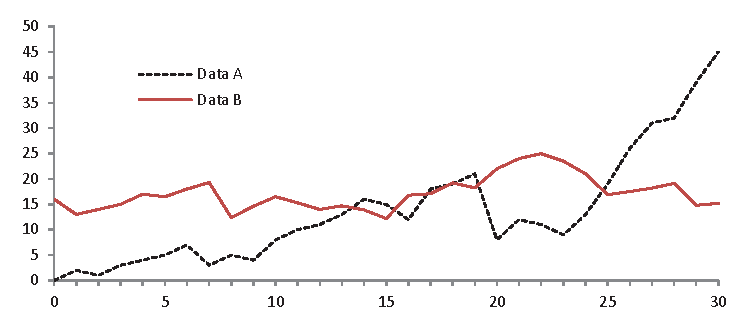
\includegraphics[width=\textwidth]{fig1.eps}
% \caption{A figure caption is always placed below the illustration.
% Please note that short captions are centered, while long ones are
% justified by the macro package automatically.} \label{fig1}
% \end{figure}

% \begin{theorem}
% This is a sample theorem. The run-in heading is set in bold, while
% the following text appears in italics. Definitions, lemmas,
% propositions, and corollaries are styled the same way.
% \end{theorem}
% %
% % the environments 'definition', 'lemma', 'proposition', 'corollary',
% % 'remark', and 'example' are defined in the LLNCS documentclass as well.
% %
% \begin{proof}
% Proofs, examples, and remarks have the initial word in italics,
% while the following text appears in normal font.
% \end{proof}
% For citations of references, we prefer the use of square brackets
% and consecutive numbers. Citations using labels or the author/year
% convention are also acceptable. The following bibliography provides
% a sample reference list with entries for journal
% articles~\cite{ref_article1}, an LNCS chapter~\cite{ref_lncs1}, a
% book~\cite{ref_book1}, proceedings without editors~\cite{ref_proc1},
% and a homepage~\cite{ref_url1}. Multiple citations are grouped
% \cite{ref_article1,ref_lncs1,ref_book1},
% \cite{ref_article1,ref_book1,ref_proc1,ref_url1}.
%
% ---- Bibliography ----
%
% BibTeX users should specify bibliography style 'splncs04'.
% References will then be sorted and formatted in the correct style.
%
% \bibliographystyle{splncs04}
% \bibliography{mybibliography}
%
% \begin{thebibliography}{8}
% \bibitem{ref_article1}
% Author, F.: Article title. Journal \textbf{2}(5), 99--110 (2016)

% \bibitem{ref_lncs1}
% Author, F., Author, S.: Title of a proceedings paper. In: Editor,
% F., Editor, S. (eds.) CONFERENCE 2016, LNCS, vol. 9999, pp. 1--13.
% Springer, Heidelberg (2016). \doi{10.10007/1234567890}

% \bibitem{ref_book1}
% Author, F., Author, S., Author, T.: Book title. 2nd edn. Publisher,
% Location (1999)

% \bibitem{ref_proc1}
% Author, A.-B.: Contribution title. In: 9th International Proceedings
% on Proceedings, pp. 1--2. Publisher, Location (2010)

% \bibitem{ref_url1}
% LNCS Homepage, \url{http://www.springer.com/lncs}. Last accessed 4
% Oct 2017
% \end{thebibliography}
\printbibliography
\end{document}
